% MosaicOpt paper - PODS theoretical draft
% Compile with: pdflatex paper.tex (twice), bibtex paper, pdflatex paper.tex (twice)

\documentclass[acmsmall,review,anonymous]{acmart}

% ---------- Packages ----------
\usepackage{amsmath}
% amssymb intentionally omitted: newtxmath (loaded by acmart) already
% provides the AMS symbol set, and the two packages collide on \Bbbk.
\usepackage{amsthm}
\usepackage{mathrsfs}
\usepackage{booktabs}
\usepackage{multirow}
\usepackage{array}
\usepackage{xcolor}
\usepackage{tikz}
\usetikzlibrary{positioning, arrows.meta, calc, shapes, fit, backgrounds, shadows.blur, decorations.pathreplacing, decorations.pathmorphing}
\usepackage[utf8]{inputenc}
\usepackage[T1]{fontenc}
\usepackage{microtype}
\usepackage{enumitem}
\usepackage{listings}
\usepackage{xspace}

% ---------- Color palette (matches presentation) ----------
\definecolor{mosaicCrimson}{HTML}{780000}
\definecolor{mosaicBlue}{HTML}{003049}
\definecolor{mosaicLightBlue}{HTML}{669BBC}
\definecolor{mosaicCream}{HTML}{FDF0D5}
\definecolor{mosaicRed}{HTML}{C1121F}
\definecolor{mosaicGray}{HTML}{8D99AE}

% ---------- Listings (SQL code blocks in Section 5) ----------
\lstset{
  basicstyle=\ttfamily\small,
  keywordstyle=\color{mosaicBlue}\bfseries,
  commentstyle=\color{mosaicGray}\itshape,
  stringstyle=\color{mosaicCrimson},
  showstringspaces=false,
  breaklines=true,
  breakatwhitespace=true,
  columns=fullflexible,
  keepspaces=true,
  numbers=none,
  frame=single,
  rulecolor=\color{mosaicLightBlue},
  framesep=4pt,
  xleftmargin=2pt,
  xrightmargin=2pt,
  aboveskip=8pt,
  belowskip=8pt,
  language=SQL
}

% ---------- Theorem-like environments ----------
\theoremstyle{plain}
\newtheorem{theorem}{Theorem}
\newtheorem{lemma}[theorem]{Lemma}
\newtheorem{corollary}[theorem]{Corollary}
\newtheorem{proposition}[theorem]{Proposition}

\theoremstyle{definition}
\newtheorem{definition}{Definition}

\newtheorem{counterexample}{Counterexample}

% Proof is built-in; redefine QED
\renewcommand{\qedsymbol}{\ensuremath{\blacksquare}}

% ---------- Notation shortcuts ----------
\newcommand{\vect}[1]{\boldsymbol{#1}}
\newcommand{\attr}[1]{\operatorname{attr}(#1)}
\newcommand{\Mem}{\mathit{Mem}}
\newcommand{\KG}{\mathit{KG}}
\newcommand{\schema}[1]{\operatorname{schema}(#1)}
\newcommand{\setof}[1]{\operatorname{set}(#1)}
\newcommand{\topK}{\operatorname{topK}}
\newcommand{\bm}[1]{\boldsymbol{#1}}

% Remark environment (used for non-blocking observations)
\theoremstyle{remark}
\newtheorem{remark}{Remark}

% ---------- CCS / Metadata ----------
\acmConference[PODS '27]{ACM SIGMOD/PODS International Conference on Management of Data / Principles of Database Systems}{2027}{}
\setcopyright{none}

\begin{CCSXML}
<ccs2012>
<concept>
<concept_id>10002951.10003317.10003331</concept_id>
<concept_desc>Information systems~Database management system engines</concept_desc>
<concept_significance>500</concept_significance>
</concept>
<concept>
<concept_id>10002951.10003317.10003338</concept_id>
<concept_desc>Information systems~Query optimization</concept_desc>
<concept_significance>500</concept_significance>
</concept>
<concept>
<concept_id>10002951.10003317.10003332</concept_id>
<concept_desc>Information systems~Database design and models</concept_desc>
<concept_significance>300</concept_significance>
</concept>
</ccs2012>
\end{CCSXML}

\keywords{agentic memory, relational algebra, query optimization, vector search, hybrid retrieval, rule-based optimizer, equational theory}

% =====================================================================
% Title
% =====================================================================
\title{MosaicOpt: An Algebraic Foundation for Agentic Memory Databases}

\author{Anonymous Author(s)}
\affiliation{
  \institution{Anonymous Institution}
  \city{Anonymous City}
  \state{Anonymous State}
  \country{Anonymous Country}}
\email{anonymous@example.com}

\begin{document}
\begin{abstract}
\noindent
Production LLM agents accumulate multi-modal memory across two timescales:
long-term facts and preferences, and short-term working context. A memory
unit typically carries text, one or more dense vector embeddings,
structured metadata, and graph relations. Useful queries against this
store are conjunctive expressions that mix all four modalities --- for
example, ``find passages about a fault-tolerance bug from the last 30
days, semantically similar to a stack trace, attributed to a known
subsystem, and connected by a derivation link to a prior incident.'' The
dominant engineering response, \emph{multi-path recall} with
application-level score fusion, has no principled semantics, no
equivalence relation over plans, and breaks down on multi-vector
conjunctions. We propose \textbf{MosaicOpt}, an \emph{algebra-first}
design that extends relational algebra with (i) a \emph{materialization}
operator $\mu$ that binds computed values (vector distances, BM25
scores) as first-class attributes, (ii) first-class vector, text, and
graph predicates, and (iii) a graph expansion operator $\Gamma$. The
optimizer is a Volcano/Cascades-style rule-based layer driven by an
\emph{equational theory} of seven foundational identities (M1--M5, G1,
G2) over the extended operators, the assumed classical
join-commutativity and join-associativity rules, derived corollaries
(M4+M1, M5+G1, A4-vector + M1, A7-symmetry, A8-regrouping) and
implied-by-definition rewrites (topK recognition, $\sigma$-$\tau$
commutation), combined with a cost-based layer that explicitly accounts
for approximation. We prove the identities, give counterexamples for
the five non-identities (N1--N5) that classical intuition suggests but
approximation or graph-traversal asymmetry breaks, and sketch a
prototype and evaluation plan. The argument is foundational: agentic
memory is a query problem, query problems benefit from algebraic
foundations, and the right foundation is an extension of relational
algebra.
\end{abstract}

\maketitle

% =====================================================================
% 1. Introduction & Motivation
% =====================================================================
\section{Introduction \& Motivation}\label{sec:intro}

Large language model (LLM) agents are no longer stateless
request--response loops. Production agents --- coding copilots, personal
assistants, autonomous research workers, multi-step planners ---
accumulate state across two timescales: \emph{long-term memory}, which
persists facts, preferences, and episodic traces across sessions; and
\emph{short-term memory}, which captures the working context of an
in-flight session, including tool-call history and intermediate
reasoning artifacts. This split is widely accepted in the
agentic-systems literature, but its consequences for the storage layer
have received less attention.

The content of agentic memory is inherently \emph{multi-modal}. A
single ``memory unit'' may carry: (i)~raw text (a chat snippet, a code
diff, a document excerpt); (ii)~one or more dense vector embeddings,
often produced by different encoders for different retrieval objectives
(e.g. semantic similarity, intent classification, code search);
(iii)~structured metadata (timestamps, source, provenance, user tags,
confidence scores); and (iv)~graph structure (entity relations such as
\texttt{derived\_from}, \texttt{cites}, \texttt{contradicts},
\texttt{member\_of}). A useful query against this store is seldom a pure
similarity lookup; it is a \emph{conjunctive} expression that mixes all
four modalities. ``Find passages about a fault tolerance bug from the
last 30 days, semantically similar to this stack trace, attributed to a
known subsystem, and connected by \texttt{derived\_from} to a previous
incident'' is representative.

The dominant engineering response is \emph{multi-path recall}: a
fan-out across specialized engines (a vector index, a full-text index,
a key--value store, a graph store), each producing a ranked candidate
list, followed by application-level score fusion and re-ranking.
Frameworks such as Mem0, Letta, Zep, and Cognee instantiate variations
of this pattern. It works, and product demonstrations are easy to find.
But the pattern has four structural weaknesses:

\begin{enumerate}[leftmargin=*]
  \item \textbf{No principled semantics.} The semantics of a fused
    query is defined by the application code that combines the
    per-channel scores. Two implementations of ``find similar memory''
    in the same product can have silently different meanings.
  \item \textbf{Heuristic optimization only.} Without an algebra, there
    is no equivalence relation over plans. The ``optimizer'' is a
    hand-tuned orchestration pipeline whose rewrites are not derived
    from a sound theory.
  \item \textbf{Fusion policy leaks into the substrate.} Score
    combination functions (e.g. weighted sum, reciprocal-rank fusion,
    learned rerankers) are application concerns; once baked into a
    query template, they are hard to change without re-engineering the
    data path.
  \item \textbf{Top-$k$ per column breaks conjunctive intent.} Each
    vector column is typically searched independently with its own
    top-$k$, then intersected. For multi-vector memories, the
    intersection of per-column top-$k$ sets is frequently empty or
    impoverished, because the columns are correlated, not redundant.
\end{enumerate}

Our position is that these problems are not implementation details;
they are symptoms of a missing foundation. \textbf{MosaicOpt} proposes
an \emph{algebra-first} design in which relational algebra is extended
with a small set of operators that make multi-modal memory queries
first-class, and in which the resulting algebra --- not application
code --- is the substrate contract between query and execution. The
optimizer becomes a \emph{rule-based} layer driven by an equational
theory (Section~\ref{sec:equational}), with a
\emph{cost-based} layer (Section~\ref{sec:impl}) choosing between
physical realizations that may legitimately differ in approximation
behaviour.

\begin{figure}[t]
  \centering
  \resizebox{\columnwidth}{!}{%
  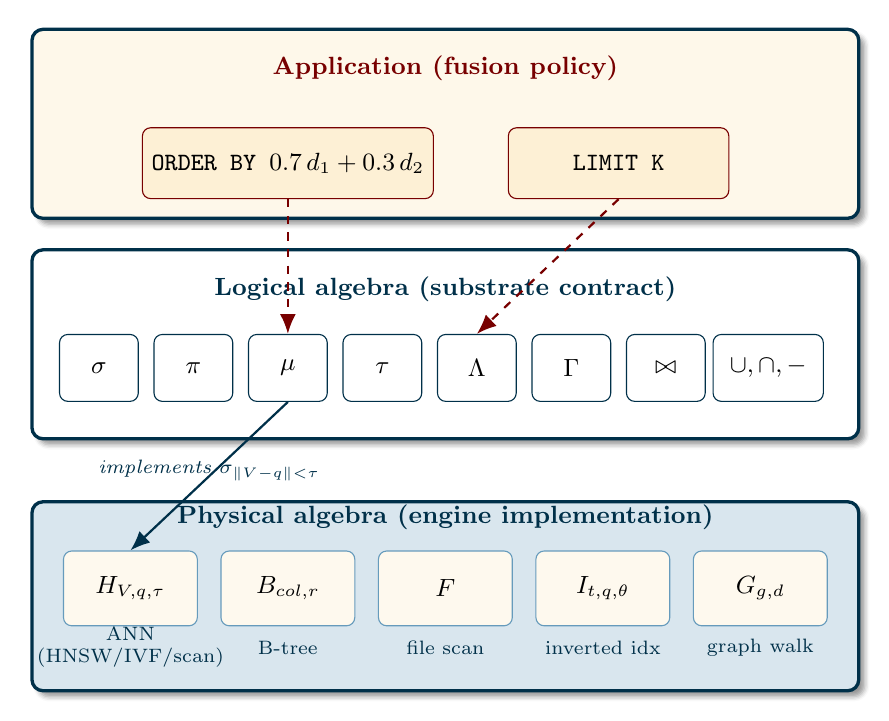
\begin{tikzpicture}[
    layer/.style={rectangle, rounded corners=4pt, draw=mosaicBlue, very thick, minimum width=10.5cm, minimum height=2.4cm, blur shadow={shadow blur steps=4}},
    appbox/.style={rectangle, draw=mosaicCrimson, fill=mosaicCream, rounded corners=3pt, minimum height=0.9cm, minimum width=2.8cm, font=\ttfamily\small},
    logbox/.style={rectangle, draw=mosaicBlue, fill=white, rounded corners=3pt, minimum height=0.85cm, minimum width=1.0cm, font=\small, inner sep=3pt},
    logbox_wide/.style={rectangle, draw=mosaicBlue, fill=white, rounded corners=3pt, minimum height=0.85cm, minimum width=1.4cm, font=\small, inner sep=3pt},
    phybox/.style={rectangle, draw=mosaicLightBlue, fill=mosaicCream!40, rounded corners=3pt, minimum height=0.95cm, minimum width=1.7cm, font=\ttfamily\small, inner sep=3pt},
    arr/.style={-{Latex[length=2.5mm,width=2mm]}, thick, color=mosaicBlue}
  ]
    % --- Top: Application layer (centered at y=4.5) ---
    \node[layer, fill=mosaicCream!50] (app) at (0,4.5) {};
    \node[font=\bfseries\small, color=mosaicCrimson] at (0,5.2) {Application (fusion policy)};
    \node[appbox] (sql1) at (-2.0,4.0) {\textbf{ORDER BY} $0.7\,d_1+0.3\,d_2$};
    \node[appbox] (sql2) at (2.2,4.0) {\textbf{LIMIT K}};

    % --- Middle: Logical algebra layer (centered at y=1.7) ---
    % 8 boxes (ρ is classical, not new — omitted from the overview; full
    % inventory in \S2.2). Set ops combined into one wide box.
    \node[layer, fill=white] (log) at (0,1.7) {};
    \node[font=\bfseries\small, color=mosaicBlue] at (0,2.4) {Logical algebra (substrate contract)};
    \node[logbox] (s1) at (-4.4,1.4) {$\sigma$};
    \node[logbox] (s2) at (-3.2,1.4) {$\pi$};
    \node[logbox] (s3) at (-2.0,1.4) {$\mu$};
    \node[logbox] (s4) at (-0.8,1.4) {$\tau$};
    \node[logbox] (s5) at (0.4,1.4) {$\Lambda$};
    \node[logbox] (s6) at (1.6,1.4) {$\Gamma$};
    \node[logbox] (s7) at (2.8,1.4) {$\bowtie$};
    \node[logbox_wide] (s8) at (4.1,1.4) {$\cup,\cap,-$};

    % --- Bottom: Physical algebra layer (centered at y=-1.5) ---
    % 5 boxes + per-box access-path sub-labels INSIDE the layer.
    \node[layer, fill=mosaicLightBlue!25] (phy) at (0,-1.5) {};
    \node[font=\bfseries\small, color=mosaicBlue] at (0,-0.5) {Physical algebra (engine implementation)};
    \node[phybox] (p1) at (-4.0,-1.4) {$H_{V,q,\tau}$};
    \node[phybox] (p2) at (-2.0,-1.4) {$B_{col,r}$};
    \node[phybox] (p3) at (0.0,-1.4) {$F$};
    \node[phybox] (p4) at (2.0,-1.4) {$I_{t,q,\theta}$};
    \node[phybox] (p5) at (4.0,-1.4) {$G_{g,d}$};
    \node[font=\scriptsize, color=mosaicBlue, align=center] at (-4.0,-2.15) {ANN\\(HNSW/IVF/scan)};
    \node[font=\scriptsize, color=mosaicBlue, align=center] at (-2.0,-2.15) {B-tree};
    \node[font=\scriptsize, color=mosaicBlue, align=center] at (0.0,-2.15) {file scan};
    \node[font=\scriptsize, color=mosaicBlue, align=center] at (2.0,-2.15) {inverted idx};
    \node[font=\scriptsize, color=mosaicBlue, align=center] at (4.0,-2.15) {graph walk};

    % Vertical arrows (Application -> Logical)
    \draw[arr, dashed, color=mosaicCrimson] (sql1.south) -- (s3.north);
    \draw[arr, dashed, color=mosaicCrimson] (sql2.south) -- (s5.north);
    % Vertical arrow (Logical -> Physical); label sits in the 0.8cm gap
    % between the two layer rectangles, well clear of all titles and boxes.
    \draw[arr] (s3.south) -- (p1.north);
    \node[font=\scriptsize\itshape, color=mosaicBlue, align=center] at (-3.0,0.1) {implements $\sigma_{\lVert V-q\rVert<\tau}$};
  \end{tikzpicture}%
  }
  \Description{Three horizontal layers, each titled at the top of its rectangle: ``Application (fusion policy)'' (cream) showing SQL \texttt{ORDER BY} and \texttt{LIMIT K} boxes; ``Logical algebra (substrate contract)'' (white) showing the eight \emph{new-or-key} logical operators $\sigma, \pi, \mu, \tau, \Lambda, \Gamma, \bowtie$, and the combined set-op family $\cup, \cap, -$ ($\rho$ is classical and omitted; full inventory in \S2.2); and ``Physical algebra (engine implementation)'' (light blue) showing the five physical operator families $H_{V,q,\tau}$ (ANN, with concrete strategy HNSW/IVF/scan chosen by the CBO), $B_{col,r}$ (B-tree), $F$ (file scan), $I_{t,q,\theta}$ (inverted index), $G_{g,d}$ (graph walk). Vertical arrows show the logical vector selection $\sigma_{\|V-q\|<\tau}$ realised by the ANN family physical operator $H_{V,q,\tau}$ whose concrete strategy (HNSW, IVF, or brute-force scan) is chosen by the cost-based optimiser.}
  \caption{Three-layer architecture of MosaicOpt.}
  \label{fig:threelayer}
\end{figure}

Figure~\ref{fig:threelayer} shows the resulting architecture.
The \emph{application} layer (top, cream) holds the fusion policy as
SQL \texttt{ORDER BY} and \texttt{LIMIT} constructs; the fusion
weights live entirely in the SQL and the substrate has no opinion on
them. The \emph{logical algebra} (middle, white) is the substrate
contract: a small set of operators over which the equational theory
is stated, including the new $\mu$ (materialization) and $\Gamma$
(graph expansion) operators. The \emph{physical algebra} (bottom,
light blue) realizes each logical operator through a concrete
access path --- HNSW, IVF, or brute-force scan for vector selection;
B-tree for structured range; inverted index for BM25; CSR /
adjacency map for graph walks. The ANN family bridge
$H_{V,q,\tau}$ (bottom of the figure) is the point at which
approximation enters the system --- a fact the logical layer hides
and the cost model (Section~\ref{sec:impl}) makes explicit.

\subsection{Why algebraic foundation?}\label{sec:intro:algebra}

Codd's relational algebra~\cite{codd1970} and Selinger's
cost-based optimizer~\cite{selinger1979} established that query
processing benefits from a formal language for what is computable
and a formal theory for what transformations preserve semantics.
The Volcano/Cascades line further showed that the algebra is the
\emph{API}: a new operator ships with its equivalence rules and cost
model, and the optimizer gains new capabilities without any central
rewrite. \textbf{An algebra is not an implementation detail; it is
the contract between query and execution.} When the algebra is
rigorous, every query language is a syntactic surface over it, every
optimizer decision is auditable, and every physical innovation is a
drop-in.

Formally, an algebra provides four things that no collection of
indexes and APIs can:

\begin{itemize}[leftmargin=*]
  \item \textbf{A language for expressive power} --- a precise
    definition of what is computable in the system, and what is not.
  \item \textbf{An equational theory} --- a body of identities that
    govern when one query plan is equivalent to another.
  \item \textbf{A cost-model framework} --- the substrate on which
    cost-based optimization rests, parameterized by the same logical
    operators the user wrote.
  \item \textbf{Composability} --- new operators can be added without
    breaking old ones, because the algebra is the integration point.
    The Cascades maxim --- \emph{the algebra is the API} --- makes
    extensibility a property of the foundation, not of the optimizer
    code.
\end{itemize}

Agentic memory is the \emph{worst case} for a ``bag of engines''
approach: it spans two timescales (long-term and short-term) with
different access patterns and consistency guarantees; its content
is genuinely multi-modal (text, multiple vector columns, structured
metadata, graph relations on the same memory unit); and the queries
that matter are \emph{conjunctive across modalities} --- a vector
range intersected with a metadata filter joined with a graph
reachability predicate. The field shows \emph{convergent evolution}:
every Agentic framework (Mem0, Letta, Zep, Cognee) has independently
reinvented the same patterns (multi-path recall, score fusion,
re-ranking) with no shared vocabulary, type system, or notion of plan
equivalence. The practical consequence is that each framework has a
different \emph{memory API} with no formal semantics, and porting a
workload requires reading source code rather than reasoning from a
specification.

\subsection{Why an algebraic foundation helps}\label{sec:intro:support}

The algebra gives database researchers and engineers a precise
substrate on which to develop new query patterns and to \emph{prove}
their correctness. A new materialization pattern or join algorithm
becomes a new operator with a documented equational theory; its
rewrite rules are \emph{derived} from the algebra, not guessed from
benchmarks. The optimizer's plan space becomes \emph{derivable}:
each new operator is added with its identities and the optimizer
gains the corresponding rewrites ``for free''. The algebra is the
\emph{shared basis} between application and engine --- an
application written once is portable across engines that share the
algebra, and an engine innovation is portable to every application
that uses the affected operator.

\subsection{Data substrate for Agentic applications}\label{sec:intro:substrate}

Four use cases illustrate the substrate requirements:
\textbf{episodic recall} (conjunctive vector + metadata + graph
queries); \textbf{cross-session fact retrieval} (multi-vector recall
with structured filters); \textbf{working context assembly} (fast
filtered recall by recency and entity); \textbf{tool-trace analysis}
(graph queries over \texttt{derived\_from} and \texttt{follows}
edges, joined with vector similarity on tool outputs). All four are
\emph{query problems} expressible as expressions over a memory store
and amenable to the same optimizer pipeline. With MosaicOpt's
algebra, the application writes its query in SQL
(Section~\ref{sec:impl}); the substrate applies M1-style rewrites to
fuse materialization with selection, M5/G1/G2 to push operators
through graph expansion, M4/M5 to push materialization through
joins, and CBO physical-operator selection. The application does not
need to know about HNSW/IVF/scan, B-tree, or inverted indexes ---
these are hidden as physical realizations of a single logical
operator; the application policy (fusion weights, thresholds,
top-$k$) stays in the SQL.

\subsection{Contributions}\label{sec:contrib}

This paper makes two contributions:

\begin{itemize}[leftmargin=*]
  \item \textbf{An extended relational algebra for agentic memory}
    (Section~\ref{sec:algebra}): a \emph{materialization} operator
    $\mu$, first-class vector/text/graph predicates, an explicit
    \emph{graph expansion} $\Gamma$, and a strict logical/physical
    separation under bag semantics.
  \item \textbf{An equational theory with proofs}
    (Section~\ref{sec:equational}): seven \emph{foundational}
    identities (M1--M5, G1, G2) over the extended operators, the
    assumed classical A1--A8 (including join commutativity and
    associativity; A1, A4 extend naturally to vector predicates),
    the derived chains M4+M1, M5+G1, A4-vector+M1, the classical
    applications A7-sym and A8-regroup, the definitional
    $\tau$-$\Lambda$-$\topK$ rewrite, the row-preserving
    $\sigma$-$\tau$ commutation, five non-identities (N1--N5) that
    approximation, graph-traversal asymmetry, or the
    traversal-vs-origin column split break, and a confluent RBO
    (Theorem~\ref{thm:rbo-confluence}).
\end{itemize}

The paper is intentionally foundational. The algebra is the
\emph{shared basis} between application and engine; a common
vocabulary will benefit the field just as it did in the relational
world. The companion SIGMOD paper~\cite{companion2026sigmod}
develops the implementation --- the SQL surface, the
rule-based and cost-based optimizers, and the prototype --- that
honors the algebraic contract proved here.

% =====================================================================
% 2. Extended Algebra (was §2 Background + §3 Extended Algebra)
% =====================================================================
\section{Extended Algebra}\label{sec:algebra}

\subsection{Background}\label{sec:background}

\subsubsection*{Relational algebra and the classical optimizer}

The relational model \cite{codd1970} and its algebra remain the
dominant formal substrate for declarative query languages; Codd
showed that a small set of operators ($\sigma$, $\pi$, product,
union, difference, rename) is sufficient for any first-order query.
The second pillar is \textbf{query optimization}: Selinger's
cost-based System~R optimizer \cite{selinger1979} enumerated
alternative orderings under a cardinality model; the \textbf{Volcano}
\cite{graefe1994} and \textbf{Cascades} \cite{graefe1995} frameworks
generalized this to a rule-based outer loop driving a cost-based
inner search, with the algebra as the API. Two ideas from this
tradition are central: an \emph{equational theory} of plan identities
is the foundation for principled rewriting, and
\emph{logical--physical separation} allows physical innovations to be
plugged in without changing semantics.

\subsubsection*{Vector search and modern IR}

Information retrieval contributed the \emph{vector space model}
\cite{salton1975} and BM25 \cite{robertson1995} as principled
relevance scoring functions. The neural era added dense embeddings
\cite{mikolov2013,reimers2019} and approximate nearest neighbour
(ANN) indexes for sub-linear search: HNSW graphs \cite{malkov2018}
are the dominant production choice, with IVF inverted files and
brute-force linear scan as alternatives. A key property of ANN
indexes is that they are \emph{approximate}: the result of an HNSW
range query is not the exact set within distance $\tau$ but an
approximation whose quality depends on the index parameters
(\texttt{ef}/\texttt{M} for HNSW, \texttt{nlist}/\texttt{nprobe} for
IVF). This approximation is invisible at the algebraic level but
central to the cost model: a high-recall ANN plan costs more than a
low-recall one, and the optimizer must trade recall against latency.

\subsubsection*{Hybrid query systems}

The last decade has produced three lines of \emph{hybrid} systems:
\textbf{vector-aware RDBMS extensions} (\texttt{pgvector}, DuckDB
\texttt{vss}, Oracle AI Vector Search) add a vector type and ANN
index at the function-call level, with no first-class identities;
\textbf{purpose-built hybrid stores} (Pinecone, Weaviate, Qdrant,
Milvus, Vespa) are vector-first with metadata filtering bolted on;
\textbf{multi-modal query languages} (SQL/MM, SPARQL with full-text,
Cypher) mix graph, text, and (in a few cases) vector. The common
pattern: every system fuses scores at the application layer rather
than extending the algebra that defines what counts as an answer.

\subsubsection*{The gap}

What is missing is an \emph{equational} view of multi-modal memory
queries in which vector distance, BM25 relevance, and graph
reachability are first-class predicates on a par with $A = c$; in
which computed values (distances, scores) are first-class attributes;
and in which the boundary between the application's \emph{fusion
policy} and the substrate's \emph{evaluation strategy} is explicit
and contractually enforced. That is the gap MosaicOpt addresses.

We extend the classical relational algebra with three new kinds of
construct: a \emph{materialization} operator $\mu$ that lifts computed
values to first-class attributes, first-class multi-modal predicates
(vector distance, BM25, graph reachability), and a \emph{graph
expansion} operator $\Gamma$. Bag semantics are used throughout,
matching SQL and avoiding the row-collapse anomalies of set semantics
in the presence of duplicate memory units; the logical/physical
separation is enforced (physical operators are introduced in
Section~\ref{sec:impl} and never appear here).

\subsection{Logical/physical separation}

Following System~R and Cascades, we treat the \emph{logical} algebra
as the substrate contract --- what the user asks for --- and the
\emph{physical} algebra as the engine contract --- how it is
evaluated. Equivalences hold in the logical algebra; physical
operators are \emph{implementations} of logical operators, and a
logical equivalence does not in general imply that two physical
realizations are interchangeable (Section~\ref{sec:equational:nonident},
N1--N3). This separation is what makes the system \emph{composable}:
the ANN family (HNSW, IVF, scan) can be added, swapped, or replaced
without changing the language the user sees.

\subsection{Operator inventory}

A \emph{logical plan} is a term over the following operators. $R$
denotes a stored base relation. $L$, $M$ denote logical plans.
$\varphi$ denotes a predicate, $e$ a materialization expression, $A$
a set of attribute names, $O$ an ordering expression, $K$ a
non-negative integer, $c$ a fresh attribute name, $g$ a graph rule
(a labelled-edge pattern), and $d$ a non-negative integer depth.

The logical operators are: \textbf{base relation} $R$;
\textbf{selection} $\sigma_\varphi(L)$ (rows satisfying $\varphi$);
\textbf{projection} $\pi_A(L)$; \textbf{materialization}
$\mu_{e\to c}(L)$ (per row, compute $e$, bind to fresh $c$);
\textbf{join} $L \bowtie_\psi M$; \textbf{set ops} $L \cup M$,
$L \cap M$, $L - M$; \textbf{rename} $\rho_{a\to b}(L)$;
\textbf{ordering} $\tau_O(L)$ and \textbf{limit} $\Lambda_K(L)$;
the abbreviation $\topK_O(L, K) := \tau_O(\Lambda_K(L))$
(the $K$ smallest rows of $L$ under $O$, a primitive we
single out because the CBO gives it a dedicated physical
realization, Section~\ref{sec:impl}); and the new
\textbf{graph expansion} $\Gamma_{g,d}(L)$ (from a node-id
attribute, traverse rule $g$ to depth $d$).

\begin{definition}[Bag semantics]\label{def:bag}
A relation is a multiset of tuples. All operators are
multiset-preserving: $\sigma$, $\mu$, $\Gamma$ preserve row
multiplicity; projection preserves multiplicity; set operations
combine multiplicities additively for $\cup$, by $\min$ for $\cap$,
and by subtraction (clamped at $0$) for $-$. $\tau_O$ produces a
totally ordered sequence; $\Lambda_K$ truncates it.
\end{definition}

Bag semantics was chosen because the substrate must be able to
express ``the same memory unit appears $N$ times'' (e.g.\ an
episodic trace where the same event is recorded with several
slightly different timestamps), and because it matches the SQL
semantics that application code already expects.

\subsection{Predicate forms}

A predicate $\varphi$ is a Boolean combination of atoms. The atom
forms are: (i)~\emph{classical} ($A = c$, $A < c$, $A > c$, $A \in
S$); (ii)~\emph{vector} ($\lVert V_a - q \rVert < \tau$ where
$V_a$ is a vector attribute, $q$ a query-time bound vector, and
$\tau \geq 0$ a threshold); (iii)~\emph{text}
($\mathrm{BM25}(t, q) > \theta$ with parameters $(k_1, b)$ from
\cite{robertson1995}); (iv)~\emph{graph}
($\mathrm{reachable}(u, v)$, $\mathrm{edge}(u, v, \ell)$); and
(v)~\emph{Boolean combinations} ($\wedge$, $\vee$, $\neg$).
\emph{Query-time bound parameters} ($q$, $\tau$, $\theta$) are
first-class values distinct from input attributes, making predicates
safely late-binding: the same algebra expression serves all query
instances, only the bound parameters change.

\subsection{Materialization: motivation, expressions, and semantics}

Inlining per-column distances in \texttt{ORDER BY} (e.g.\
\texttt{ORDER BY} $\lVert V_a - q_a \rVert + \lVert V_b - q_b
\rVert$) is permitted by SQL extensions, but it forces the
application to write the distance expression everywhere it is used
and leaves the optimizer no room to share computation between a
\texttt{WHERE} filter and an \texttt{ORDER BY} rank. The
materialization operator $\mu_{e \to c}(L)$ binds a per-row
expression $e$ to a fresh attribute name $c$, making the
materialized value referenceable by downstream $\sigma$, $\pi$,
$\tau$, and $\mu$ (see
Section~\ref{sec:example} for an example). Valid forms of $e$ are
classical ($A + B$, $f(A)$), vector ($\lVert V_a - q \rVert$),
text ($\mathrm{BM25}(t, q)$), and Boolean or arithmetic combinations.
The fresh-name condition (Def.~\ref{def:fresh}) requires $c$ to be
absent from $\schema{L}$; $\rho$ is provided to free names.

\begin{definition}[Fresh-name condition]\label{def:fresh}
$c$ in $\mu_{e\to c}(L)$ must not already appear in $\schema{L}$.
$\rho$ is provided to free names if needed.
\end{definition}

The semantics is the multiset $\{\, r \oplus \{c \mapsto e(r)\} :
r \in L \,\}$. If $e(r)$ is undefined (e.g.\ distance to a null
vector), the row is dropped --- consistent with SQL's \texttt{NULL}
handling and essential for safety in the presence of missing
embeddings.

\subsection{Graph expansion}

$\Gamma_{g,d}(L)$ takes a plan whose rows contain a node-id attribute
($u$, say) and a graph attribute, applies graph rule $g$ up to depth
$d$, and returns the \emph{target} nodes of those traversals (joined
with the originating row). The depth is inclusive of intermediate
hops. $g$ is a labelled-edge pattern: a regular expression over edge
labels, evaluated against the graph. The graph itself is supplied as
a relation-valued attribute; the expansion is a join between $L$ and
the traversal result.

$\Gamma$ is intentionally narrow. We do not attempt to encode path
queries as selection predicates; this keeps the operator set small
and the rewrite theory tractable (Section~\ref{sec:equational}, G1,
G2). Path information can be recovered by a $\mu$ that records the path
taken.

\begin{remark}[$\Gamma$ identity at depth $0$]\label{rem:gamma-id}
$\Gamma_{g,0}(L) = L$ for any rule $g$ and any plan $L$ --- at
depth zero no traversal is performed, so the expansion is the
identity on rows. The rule $g$ is irrelevant at $d=0$. This is the
unit of $\Gamma$ composition under the G2 transitivity rule of
Section~\ref{sec:equational:foundational}: for any $d_1, d_2$,
$\Gamma_{g,d_1}(\Gamma_{g,d_2}(L)) = \Gamma_{g,d_1+d_2}(L)$, and
the $d=0$ case is the trivial instance $\Gamma_{g,0}(L) = L$.
\end{remark}

\subsection{Example queries}\label{sec:example}

We use a single running example throughout. Let $\Mem$ be a memory
relation with schema
$\Mem(\mathit{id}, \mathit{text}, \mathit{ts}, \vect{emb}, \vect{emb\_alt},
\mathit{user}, \mathit{subsystem})$ and $\KG$ a graph relation
$\KG(\mathit{src}, \mathit{dst}, \mathit{label})$. The query ``find
similar passages in the fault-tolerance subsystem from the last 30
days, ranked by a weighted sum of two distances, top 10'' is
\begin{align*}
Q_1 &= \Mem, \\
Q_2 &= \sigma_{\mathit{subsystem} = \mathrm{`ft'} \wedge \mathit{ts} > \mathrm{now}() - 30d}(Q_1), \\
Q_3 &= \mu_{\lVert\vect{emb} - \vect{q}_1\rVert \to d_1}\;
        \mu_{\lVert\vect{emb\_alt} - \vect{q}_2\rVert \to d_2}(Q_2), \\
Q_4 &= \sigma_{d_1 < \tau_1 \wedge d_2 < \tau_2}(Q_3), \\
Q_5 &= \tau_{0.7\cdot d_1 + 0.3\cdot d_2}(Q_4), \\
Q_6 &= \Lambda_{10}(Q_5).
\end{align*}
The algebra's job is to make this expression \emph{rewriteable}
--- to compute $d_1, d_2$ only on rows that survive the filter
(M1) and to enable top-$K$ early termination (the
$\tau\,\Lambda\,/\,\topK$ recognition in
Section~\ref{sec:equational:convergent}). A graph-aware
variant intersects the result with a two-hop $\Gamma$ expansion
$R_2 = \Gamma_{\mathit{label}=\mathrm{`derived\_from'},\, d=2}(R_1)$.

% =====================================================================
% 4. Equational Theory: Identities and Non-Identities
% =====================================================================
\section{Equational Theory}\label{sec:equational}

The optimizer is driven by an \emph{equational theory} of identities
over logical plans, together with the \emph{non-identities} that
classical intuition suggests but approximation, graph-traversal
asymmetry, or the traversal-vs-origin column split break --- so the
optimizer knows not to apply them. This section unifies both: the
\emph{seven} genuinely-new foundational identities that the extended
operators license (M1--M5, G1, G2), the assumed classical identities
that the RBO uses for join reordering (A7, A8, alongside
A1--A6; A1, A4 apply to vector predicates by substitution), the
derived chains and classical applications (M4+M1, M5+G1,
A4-vector+M1, A7-sym, A8-regroup), the implied-by-definition
$\tau\,\Lambda\,/\,\topK$ and $\sigma$-$\tau$ rules, the
non-identities (N1--N5) with counterexamples, and the convergent
rewriting analysis.

\subsection{Overview}\label{sec:equational:overview}

The theory plays two roles. \emph{First}, it is the foundation for
the RBO (Section~\ref{sec:impl}): every rewrite is justified by an
identity (M1--M5, G1, G2, or a derived combination M4+M1,
M5+G1, A4-vector+M1, A7-symmetry, A8-regrouping, or the implied
$\sigma$-$\tau$ rewrite and $\tau\,\Lambda\,/\,\topK$
recognitions), so the optimizer's behaviour is auditable.
\emph{Second}, the non-identities (N1--N5) discipline the
optimizer against rewrites that hold in classical relational
algebra but break under approximation, asymmetric physical costs,
or graph-traversal semantics. The cost model is responsible for the
physical cost of every rewrite; the equational theory is responsible
for its \emph{correctness}. Both are first-class data: the RBO loads
them, the cost model consults them, and the executor relies on them
for safety of adaptive re-planning.

\subsection{Foundational axioms}\label{sec:equational:foundational}

The seven identities below are the \emph{new} algebraic content
licensed by the extended operators; each is stated with its
applicability conditions and a pointer to the proof (full
proofs in Appendix~A.1). We do \emph{not} state as separate
axioms the identities that are \emph{implied} by other operators
or by classical RA: classical join commutativity (A7) and join
associativity (A8) are assumed (they are in every RA textbook,
and the RBO uses them as join-reordering moves to enumerate the
$O(n!)$ join orderings of Section~\ref{sec:impl}); the
$\tau\,/\,\Lambda\,/\,\topK$ family is closed by the definition
$\topK_O(L, K) := \tau_O(\Lambda_K(L))$ from
Section~\ref{sec:algebra} and the
$\sigma$-$\tau$ commutation follows immediately from the
row-preserving semantics of $\sigma$ and $\tau$ (Def.~\ref{def:bag}).
A handful of other classical identities (selection through
intersection/difference, projection through set operations, join
through set operations) are likewise assumed.

\begin{theorem}[M1 --- Selection commutes with materialization on the materialized column]\label{thm:m1}
Where $c$ is a fresh attribute name and $e$ is an expression
depending only on attributes of $L$:
\[
\sigma_{c < \tau}\, \mu_{e \to c}(L) \;=\; \mu_{e \to c}\, \sigma_{e < \tau}(L).
\]
\end{theorem}

(\textit{Proof in Appendix A.1.})

\begin{theorem}[M2 --- Materialization is commutative]\label{thm:m2}
For fresh names $c_1, c_2$ and expressions $e_1, e_2$ depending
only on $L$'s attributes (and not on each other's outputs):
\[
\mu_{e_1 \to c_1}\, \mu_{e_2 \to c_2}(L)
\;=\;
\mu_{e_2 \to c_2}\, \mu_{e_1 \to c_1}(L).
\]
\end{theorem}

(\textit{Proof in Appendix A.1.})

\begin{theorem}[M3 --- Materialization through projection]\label{thm:m3}
For fresh $c$ and expression $e$ depending only on attributes in $A$:
\[
\mu_{e \to c}\, \pi_A(L) \;=\; \pi_{A \cup \{c\}}\, \mu_{e \to c}(L).
\]
\end{theorem}

(\textit{Proof in Appendix A.1.})

\begin{theorem}[M4 --- Materialization pushdown through join]\label{thm:m4}
Where $e$ depends only on attributes of $L$ and $c$ is a fresh
attribute name:
\[
\mu_{e \to c}\, (L \bowtie_\psi M)
\;=\;
(\mu_{e \to c}(L)) \bowtie_\psi M.
\]
\end{theorem}

(\textit{Proof in Appendix A.1.})

\begin{theorem}[M5 --- Materialization pushdown through graph expansion]\label{thm:m5}
Where $e$ depends only on attributes of $L$, $c$ is fresh and is
not the graph rule's node-id attribute (Def.~\ref{def:fresh}):
\[
\mu_{e \to c}\, \Gamma_{g, d}(L)
\;=\;
\Gamma_{g, d}\, \mu_{e \to c}(L).
\]
This is the $\mu$-counterpart of G1 and the rewrite the RBO
generates for graph queries that materialize a per-origin
attribute (e.g.\ a distance to a fixed query point) and then
expand. The two sides produce the same multiset of
$(r, v, c)$ tuples; the cost differs because the LHS computes
$e$ on every traversal row while the RHS computes $e$ on every
origin row. When $|\Gamma_{g,d}(L)| > |L|$ (the typical case for
$d \geq 1$ and a non-trivial graph), the RHS is cheaper, and
the CBO picks it.
\end{theorem}

(\textit{Proof in Appendix A.1.})

\begin{theorem}[G1 --- Selection pushdown through graph expansion]\label{thm:g1}
Where $\varphi$ references only attributes of $L$ (and not
attributes of the graph rule's traversal result):
\[
\sigma_\varphi\, \Gamma_{g, d}(L) \;=\; \Gamma_{g, d}\, \sigma_\varphi(L).
\]
\end{theorem}

(\textit{Proof in Appendix A.1.})

\begin{theorem}[G2 --- Graph expansion is transitive]\label{thm:g2}
Let $g_1, g_2$ be graph rules over the same graph attribute
with disjoint label sets. If $g_1$'s traversal-result
attribute and $g_2$'s source attribute are disjoint (no
intermediate node of $g_2$ is a valid origin of $g_1$),
then the composition $g_1 ; g_2$ satisfies:
\[
\Gamma_{g_1, d_1}\, \Gamma_{g_2, d_2}(L) \;=\;
\Gamma_{g_1;g_2,\, d_1+d_2}(L).
\]
G2 lets the RBO collapse nested $\Gamma$s into a single
expansion at depth $d_1 + d_2$ --- ``two \texttt{derived\_from}
hops'' becomes ``one \texttt{derived\_from} ;
\texttt{derived\_from} hop''.
\end{theorem}

(\textit{Proof in Appendix A.1.})

\subsection{Derived identities}\label{sec:equational:derived}

Composing the foundational axioms and the assumed classical
identities yields additional rewrites:
\begin{itemize}[leftmargin=*]
  \item \textbf{A4-vector (in code: \texttt{J1}).} A4 specialized
    to a vector predicate --- $\sigma_{\lVert V_a - q \rVert < \tau}\,
    (L \bowtie_\psi M) = (\sigma_{\lVert V_a - q \rVert < \tau}(L))
    \bowtie_\psi M$ when $V_a \in \schema{L}$ --- is what the CBO
    applies on the conjunctive multi-vector case. A1 likewise
    specializes to two vector predicates on distinct columns.
    Neither is a new algebraic identity --- both follow from
    A1/A4 by predicate substitution --- but the codebase keeps
    them as named redex patterns (\texttt{V1}, \texttt{J1}) so the
    RBO can match them explicitly.
  \item \textbf{A7-symmetry (reverse join).} A7 in the reverse
    direction; the CBO chooses the cheaper side per
    Theorem~\ref{thm:n2}.
  \item \textbf{A8-regrouping (different join parenthesization).}
    A8 enumerates the $O(n!)$ join orderings; the CBO picks the
    best. (For two joins, A8 is degenerate; for $n \geq 3$ it
    unlocks the full plan space.)
\end{itemize}
\textbf{A4-vector+M1} pushes a join-side vector selection below a
materialization binding the same distance (apply A4 then M1).
\textbf{M4+M1} reorders a join-side materialization so the
expensive per-row computation runs only on rows that survive the
join's downstream filter (apply M4 then M1) --- the converse of
A4-vector+M1 and the rewrite that powers the
Section~\ref{sec:impl} running example. \textbf{M5+G1} reorders
a graph query with both row-level filter and materialization
(apply G1 then M5).
\textbf{topK} and the $\sigma$-$\tau$ commutation are both
\emph{implied-by-operator-definition} rules: $\topK$ by
$\topK_O(L, K) := \tau_O(\Lambda_K(L))$ from
Section~\ref{sec:algebra}, and $\sigma$-$\tau$ commutation by the
row-preserving semantics of $\sigma$ and $\tau$
(Def.~\ref{def:bag}); the RBO applies them in the zero-weight
post-$w$ rewriting pass. The algebra is closed under composition
--- A1--A8 plus the seven foundational axioms plus the rewrite
rules above suffice to cover the optimization of every plan whose
operators draw from the Section~\ref{sec:algebra} inventory.

\subsection{Non-identities and counterexamples}\label{sec:equational:nonident}

Some rules that look natural in a relational setting \textbf{do not
hold} in the extended algebra. We document these explicitly so the
optimizer knows not to apply them. The same logical plan in two
realizations can have different outputs; the optimizer must treat
this as a \emph{cost} phenomenon, not a \emph{correctness} phenomenon.

\subsubsection{N1: Approximation breaks logical equivalence}

\begin{theorem}[N1 --- ANN approximation breaks logical equivalence]\label{thm:n1}
Logical $\sigma_{\lVert V-q\rVert<\tau}(R)$ is exactly defined;
physical $H_{V, q, \tau}(R)$ under HNSW or IVF is approximate
(misses true neighbours, may include non-neighbours). A logical
equivalence does not imply that two physical realizations
preserve it.
\end{theorem}

\begin{counterexample}\label{ce:n1}
A row with $\lVert\vect{v}-\vect{q}\rVert = 0.99\tau$ may be
missed by a small-\texttt{ef} HNSW but returned by an exact linear
scan: two valid implementations of the same logical selection
disagree. The optimizer must model approximation as a first-class
\emph{cost dimension} with quantified recall/precision.
\end{counterexample}

\subsubsection{N2: Similarity join asymmetry}

\begin{theorem}[N2 --- Similarity join asymmetry]\label{thm:n2}
$R \bowtie_{\lVert V_a-V_b\rVert<\tau} S$ and
$S \bowtie_{\lVert V_b-V_a\rVert<\tau} R$ are logically
equivalent; the two physical sides are not interchangeable in cost.
\end{theorem}

\begin{counterexample}\label{ce:n2}
Probing a $10^6$-row HNSW on $R$ with each row of a $10^3$-row $S$
costs $10^3$ probes; the reverse (probe $S$ for each row of $R$)
costs $10^6$ --- three orders of magnitude apart. The RBO
generates both orderings; only the CBO can decide which is
cheaper.
\end{counterexample}

\subsubsection{N3: Limit and order do not distribute over union}

\begin{theorem}[N3 --- Limit and order do not distribute over union]\label{thm:n3}
$\Lambda_K\, \tau_O\, (R \cup S) \;\neq\; \Lambda_K\, \tau_O(R) \cup
\Lambda_K\, \tau_O(S)$ in general.
\end{theorem}

\begin{counterexample}\label{ce:n3}
Let $R$ and $S$ each contain 100 rows with a single scoring
column; draw $R.\mathrm{score} \sim \mathcal{U}([0,1])$ and
$S.\mathrm{score} \sim \mathcal{U}([9,10])$. The LHS
$\Lambda_5\,\tau\,(R \cup S)$ returns the 5 rows with the
\emph{globally} smallest scores --- all from $R$, with scores
in $[0, 0.05]$. The RHS $\Lambda_5\,\tau(R) \cup \Lambda_5\,\tau(S)$
returns the 5 smallest of $R$ \emph{plus} the 5 smallest of $S$
--- 10 rows total, spanning the disjoint score ranges. The
identity would be useful for distributed top-$K$ (each shard
returns its local top-$K$ then unions), but does not hold; the
distributed top-$K$ problem is precisely about
Section~\ref{sec:open:distributed}'s threshold-exchange protocol.
\end{counterexample}

\subsubsection{N4: Materialization through graph expansion fails on traversal columns}

\begin{theorem}[N4 --- $\mu$ through $\Gamma$ on the traversal column]\label{thm:n4}
M5 (Theorem~\ref{thm:m5}) requires $e$ to depend only on
\emph{origin} attributes of $L$. When $e$ references the
traversal-result attribute produced by $\Gamma$, $\mu$ does
\emph{not} commute with $\Gamma$:
\[
\mu_{e \to c}\, \Gamma_{g, d}(L) \;\neq\;
\Gamma_{g, d}\, \mu_{e \to c}(L)
\]
in general when $e$ depends on the traversal result.
\end{theorem}

\begin{counterexample}\label{ce:n4}
Let $L$ have rows $(\mathit{id}, \vect{emb})$ and let
$\Gamma_{\mathrm{follows},1}$ produce an additional
$\vect{followed\_emb}$ attribute. Take
$e := \lVert \vect{followed\_emb} - \vect{q} \rVert$, a
distance to the \emph{followed} node's embedding. The LHS
$\mu_{e \to c}\,\Gamma(L)$ materializes $c$ against the
followed-node vector; the RHS
$\Gamma_{\mathrm{follows},1}\,\mu_{e \to c}(L)$ materializes
$c' = \lVert \vect{emb} - \vect{q} \rVert$ against the
\emph{origin} vector (the followed-attribute is not yet
bound) and then expands --- the two multisets compute
different distances row-by-row. N4 blocks the RBO from
applying M5 when the materialization expression reads a
traversal-attribute column.
\end{counterexample}

\subsubsection{N5: Limit and order do not commute with graph expansion}

\begin{theorem}[N5 --- $\Lambda$/$\tau$ do not commute with $\Gamma$]\label{thm:n5}
$\Lambda_K\, \tau_O\, \Gamma_{g, d}(L) \;\neq\;
\Gamma_{g, d}\, \Lambda_K\, \tau_O(L)$ in general.
\end{theorem}

\begin{counterexample}\label{ce:n5}
Let $L$ have 1000 origin rows with a $\mathit{score}$ column
and let $\Gamma_{\mathrm{cites},1}$ expand each origin to a
variable $1 \leq n_i \leq 50$ of citing nodes. The LHS
$\Lambda_{10}\, \tau_{\mathit{score}}(\Gamma(L))$ returns
the 10 rows of the expansion with the globally smallest
$\mathit{score}$ (some origins may contribute several
winners; some origins none). The RHS
$\Gamma(\Lambda_{10}\, \tau_{\mathit{score}}(L))$ first picks
the 10 origin rows with the smallest $\mathit{score}$ and
then expands each --- returning up to $10 \cdot 50 = 500$
rows that all share those 10 origins. The two multisets
differ in cardinality and in content: the LHS asks ``across
all reachable nodes, which $K$ score lowest?''; the RHS
asks ``among the $K$ highest-scoring origins, which nodes
are reachable?''. N5 blocks the RBO from pushing $\Lambda$
or $\tau$ through $\Gamma$; the cost model of
Section~\ref{sec:impl} reflects this by giving
$\tau\, \Lambda\, \Gamma$ a substantially higher cost than
$\Gamma\, \tau\, \Lambda$ when the expansion fan-out is large.
\end{counterexample}

\subsection{Convergent rewriting}\label{sec:equational:convergent}

The equational theory can be oriented into a \textbf{rewriting
system} $\to_{\mathrm{RBO}}$ on logical plans; the optimizer of
Section~\ref{sec:impl} is an interpreter for $\to_{\mathrm{RBO}}$.
Define the weight $w(P) = \alpha s(P) + \beta r(P) + \gamma p(P)$
where $s$ counts $\sigma$s on $\mu$-bound attributes
(M1-fixable), $r$ counts redundant $\mu$s, and $p$ counts $\pi$s
that drop needed attributes (M3-fixable). \textbf{M1, M3, M4, G1
strictly decrease $w$}, and \textbf{M2, M5, G2, and the implied
$\sigma$-$\tau$ reordering are zero-weight rewrites}: M2 is a
$\mu$-reordering that preserves $s, r, p$ and is bounded by the
$k!$ orderings on $k$ materializations; M5 is a $\mu$-$\Gamma$
reordering that preserves $s, r, p$ and is bounded by the number
of $\mu$-$\Gamma$ inversions in $P$; \textbf{G2 is a
$\Gamma$-$\Gamma$ collapse} that preserves $s, r, p$ and is
bounded by the number of nested-$\Gamma$ inversions in $P$ (one
collapse per nesting, hence the depth $d$ of the result); the
$\sigma$-$\tau$ rewrite (implied by the row-preserving semantics
of $\sigma$ and $\tau$) preserves $s, r, p$ and is bounded by the
number of $\sigma$-$\tau$ inversions in $P$. The M1/M3/M4/G1
sub-rewriting system terminates by the strict decrease of $w$;
once $w$ reaches a local minimum under those four rules, only
the zero-weight rewrites remain, and each terminates by its
bounded inversion count. The CBO-applied $\topK$ recognition
($\tau_O\,\Lambda_K \leftrightarrow \topK_O$ per
$\topK_O(L, K) := \tau_O(\Lambda_K(L))$) is a definitional
rewrite that the CBO applies as a physical-realization choice;
it is in one-to-one correspondence with its inverse and so
trivially terminates. The critical pairs from overlapping redexes
(M1$\cap$M1, M1$\cap$M4, M1$\cap$G1, M1$\cap$M5,
M4$\cap$G1, M4$\cap$M5, M5$\cap$G1, G1$\cap$A4, G2$\cap$G2,
G2$\cap$G1, G2$\cap$M5, M2$\cap$M1, M2$\cap$M5, $\sigma$-$\tau$
$\cap$ M1, $\sigma$-$\tau$ $\cap$ M3) all join by further
rewrites, giving local confluence. (The A7/A8 classical
join-reordering identities and the $\tau\,\Lambda\,/\,\topK$
definitional rewrite are included for completeness; in practice
the CBO applies the $\tau\,\Lambda\,/\,\topK$ rewrite directly as
a physical realization choice, and the RBO applies A7/A8 as
join-reordering moves.) By Newman's lemma \cite{newman1942},
termination + local confluence imply confluence and a unique
normal form:

\begin{theorem}[RBO Confluence]\label{thm:rbo-confluence}
For any starting logical plan $P$ and any two RBO rewrite sequences
$P \to^*_{\mathrm{RBO}} P^*$ and $P \to^*_{\mathrm{RBO}} P^{**}$,
there exists a plan $P^\infty$ with $P^* \to^*_{\mathrm{RBO}}
P^\infty$ and $P^{**} \to^*_{\mathrm{RBO}} P^\infty$. The normal
form is unique: it depends only on $P$, not on rewrite order.
\end{theorem}

(\textit{Proof in Appendix A.2.})

Theorem~\ref{thm:rbo-confluence} is the formal correctness guarantee
of the RBO --- the optimizer can be implemented as a simple greedy
loop (apply any rule that decreases $w$) without losing correctness.
The CBO inherits confluence ``for free'': its search is over the
unique canonical form, so its choice of physical realization is
well-defined and reproducible.

% =====================================================================
% 5. Implementation: A Brief Note
% =====================================================================
\section{Implementation: A Brief Note}\label{sec:impl}

The equational theory of Section~\ref{sec:equational} is the
foundation on which an implementation rests. The companion
SIGMOD paper~\cite{companion2026sigmod} develops the full
implementation: the SQL/MM-style surface that desugars into the
algebra, the rule-based optimizer that applies the equational
rewrites, the cost-based physical-operator selector, and the
prototype built on DuckDB, \texttt{faiss-cpu}, and
\texttt{rank\_bm25}. The present paper restricts itself to the
algebraic content; we record here only the design choices that
\emph{constrain} the equational theory (rather than describe the
implementation in detail).

\paragraph{Logical/physical separation.}
The cost model and physical operator catalog are
\emph{separate} from the equational theory. The identities
hold for any choice of physical realization; the CBO picks a
realization from a precomputed physical catalog. The cost model
is a 4-tuple $(\mathit{io}, \mathit{cpu}, \mathit{mem},
\mathit{approx}) \in \mathbb{R}^4_{\geq 0}$, the fourth component
quantifying the recall penalty of an approximate ANN strategy.
The cost model is used to \emph{search} the plan space, not to
\emph{define} the equivalence class.

\paragraph{TopK recognition.}
The $\tau\, \Lambda$ family is closed by the definition
$\topK_O(L, K) := \tau_O(\Lambda_K(L))$; the rewrite
$\tau_O\,\Lambda_K \leftrightarrow \topK_O$ is applied by the CBO
as a physical-realization choice, not as a logical RBO rewrite.
This definitional rewriting is one-to-one with its inverse, so it
trivially terminates; the RBO's confluent ARS does not depend on it.

\paragraph{SQL surface.}
The SQL/MM-style surface --- \texttt{IS NEAR}, \texttt{MATCHES},
\texttt{IS REACHABLE} --- is the application's primary interface.
Its desugaring into the algebra is total and semantics-preserving,
so every SQL query expresses a plan in the algebra, and every
plan in the algebra has a SQL rendering. The design rationale
(downstream of this paper's algebraic content) is that the SQL
extension must read as a \emph{first-class} language construct, not
as a function-style abbreviation, so the substrate is committed
to understanding the construct and to applying the equational
theory to it. The companion SIGMOD paper develops the desugaring
rules in full and reports the four experiments that validate
the end-to-end pipeline.

\paragraph{Boundary with the implementation.}
The implementation is open-source and is the primary artifact
that the SIGMOD paper analyzes. The equational theory in the
present paper is the \emph{contract} that the implementation
honors: every SQL query routed through the optimizer must
produce a result equal (as a multiset) to the result the
algebra evaluates, and the optimizer's rewrite sequence must
terminate at a unique normal form (Theorem~\ref{thm:rbo-confluence}).

\section{Discussion}\label{sec:related}

\subsection{Related work}

We identify the lineage of MosaicOpt precisely --- the goal is not
to enumerate all related work but to make clear what is novel.

\paragraph{Classical relational algebra.}
MosaicOpt inherits from Codd's relational algebra
\cite{codd1970} (the small operator set that expresses any
first-order query, refined over time and crystallized in SQL) and
from the Selinger/Volcano/Cascades line
\cite{selinger1979,graefe1994,graefe1995} (cost-based
optimization, extensible rule-based rewriters, the maxim that the
algebra is the API). These two pillars are unchanged; what
MosaicOpt adds is (i) a set of new identities (M1--M5, G1, G2)
for the extended operators, and (ii) an explicit
convergent-rewriting analysis
(Section~\ref{sec:equational:convergent}).

\paragraph{Algebraic extensions of the relational model.}
MosaicOpt continues a long lineage of ``extend the algebra, prove
identities'' work: \textbf{nested} relational algebra
\cite{thomasfischer1986} adds set-valued attributes (MosaicOpt
adds first-class materialization); \textbf{object-relational}
extensions \cite{beech1988} add user-defined types; \textbf{temporal}
algebras \cite{tuzhilinclifford1990,snodgrass1995} add time-aware
predicates; \textbf{semi-structured} algebras
\cite{fernandezsimeonwadler2000} add tree-structured data and
bisimulation-style identities. MosaicOpt extends in a
\emph{new direction} --- multi-modal (text + vector + graph) in the
context of agentic memory --- and provides, in one place, a SQL
surface and a proven equational theory the prior extensions did
not.

\paragraph{Equational theories in query optimization.}
The classical identities (selection pushdown, join commutativity,
projection pushdown) have been in the optimizer's arsenal since
System~R. The convergent-rewriting analysis of
Section~\ref{sec:equational:convergent} draws on Newman's lemma
\cite{newman1942}, Huet's critical-pair analysis \cite{huet1980},
and the Terese textbook \cite{terese2003}. The closest database
prior is Atzeni and Torlone's \cite{atzenitorlone1996} algebraic
treatment of schema and view integration across heterogeneous
data models, whose algebraic-rewriting pattern is identical.
MosaicOpt's analysis is, to our knowledge, the first such analysis
for an algebra that includes vector, text, and graph operators.

\subsection{Hybrid query algebra (recent)}

The last decade has produced a sustained effort to bring vector and
relational together, but with very few \emph{theoretical}
contributions. The systems are numerous; the algebras are few:
\textbf{vector-aware RDBMS extensions} (PostgreSQL
\texttt{pgvector}, DuckDB \texttt{vss}, Oracle AI Vector Search)
add a vector type, an ANN index, and distance predicates at the
function-call level --- systems, not theories;
\textbf{purpose-built hybrid stores} (Pinecone, Weaviate, Qdrant,
Milvus, Vespa) are vector-first with metadata filtering bolted on
and expose no named identities; \textbf{multi-modal query languages}
(SQL/MM, SPARQL with full-text, Cypher) mix graph, text, and
(in a few cases) vector, but SPARQL's vector fusion remains open.
The common pattern: every system fuses scores at the application
layer. MosaicOpt's contribution is to make the fusion
\emph{first-class}: a materialization expression is a syntactic
construct, the optimizer sees it, the cost model accounts for it,
and the equational theory of Section~\ref{sec:equational} applies.

% =====================================================================
% 10. Open Theoretical Problems
% =====================================================================
\subsection{Open theoretical problems}\label{sec:open}

Each layer of the algebra, equational theory, and optimizer opens
new theoretical problems that the algebra makes accessible but does
not yet solve. We list the most important.

\paragraph{Complexity of CBO.}\label{sec:open:complexity}
Classical join ordering is solvable in $O(n^2)$ for left-deep trees
\cite{selinger1979} but NP-hard for bushy trees
\cite{ibarakikameda1984,pellenkoft1996}. When the cost model
also ranges over probabilistic predicates, the problem becomes
strictly harder still \cite{dalvi2007}. The CBO of
Section~\ref{sec:impl} adds three new dimensions:
(i)~\emph{vector selections} as first-class operators contribute a
\emph{continuous} (\texttt{ef}-, \texttt{nprobe}-parameterized)
choice, not a discrete one; (ii)~\emph{graph expansion} has a
direction-parameterized realization whose cost depends on
\emph{graph density} at the expansion point; (iii)~\emph{materialization
sharing} is a partition problem --- each $\mu$ may be shared with
another $\mu$ or kept distinct, and the CBO must decide. We
conjecture NP-hardness in the general case and conjecture
polynomial-time subclasses for queries that bound the number of
graph expansions, the depth of materialization sharing, and the
cardinality of physical realizations per operator. Identifying
these subclasses --- and proving the tractable/intractable
boundary --- is a central open problem.

\paragraph{Adaptive optimization.}
The cost model is static --- evaluated once at planning time ---
but wrong in practice (cardinality drifts, ANN recall varies with
the query, BM25 selectivity is hard to predict). \emph{Adaptive
optimization} \cite{graefe1994} must interact correctly with the
algebra's convergent rewriting: the re-planned logical plan must be
a ``refinement'' of the original, and any non-normal-form subplan
the CBO switches to must later re-rewrite --- a property we
conjecture holds locally to the switched subtree.

\paragraph{Distributed execution.}\label{sec:open:distributed}
A distributed extension requires a network-cost model, partition-aware
physical operators (e.g.\ a partition-aware $\mathrm{TopK}$ that
respects N3), and an extension of the equational theory to reason
about partitioning. The asymmetry is that graph expansion $\Gamma$ is
harder to parallelize than vector selection --- a graph expansion must
traverse edges across partition boundaries, while a vector selection
is partitioned by the index itself. The cost of $\Gamma_{g,d}$ is a
function of the partition structure, not just the graph size.

\paragraph{Write paths and memory evolution.}\label{sec:open:write}
The algebra is read-only. A write algebra must model
(i)~\emph{incremental materialization updates} (when a base row
changes, every $\mu$ that depends on it must be invalidated or
recomputed; the equational theory gives the semantics,
incremental maintenance is harder);
(ii)~\emph{index updates} (ANN and inverted indexes must stay
consistent with the base data); and
(iii)~\emph{cost model drift} (cardinality and selectivity
parameters drift and need re-calibration). Writes are the
largest open problem in the paper.

\subsection{Limitations and out-of-scope}

\begin{itemize}[leftmargin=*]
  \item \textbf{No new physical data structures.} ANN indexes,
    B-trees, and inverted indexes are external; the contribution is
    the \emph{algebraic} use of these primitives, not their internal
    design. A learned-index primitive \cite{kraska2018} is a drop-in
    replacement in the bridge table.
  \item \textbf{No new learning-based optimization.} The
    MosaicOpt contribution is at the \emph{logical} layer; a learned
    optimizer can \emph{instantiate} the cost model without touching
    the algebra.
  \item \textbf{No new transaction model.} The algebra is read-only
    and single-node; transactional and distributed extensions are
    out of scope and addressed in the open problems above.
\end{itemize}

These are \emph{scope choices} that keep the contribution focused
on the algebraic foundation.

% =====================================================================
% Acknowledgements
% =====================================================================
\begin{acks}
This draft builds on the project design brief
(\texttt{docs/brief.md}). Sections~\ref{sec:algebra}--\ref{sec:equational}
derive from the brief's algebra-design decisions. The authors thank
the open-source communities of HNSW (\texttt{hnswlib}), Tantivy,
DuckDB, and Cascades-style optimizers for the building blocks that
make the prototype tractable.
\end{acks}

% =====================================================================
% References
% =====================================================================
\begin{thebibliography}{99}

\bibitem{companion2026sigmod}
Anonymous.
\newblock The MosaicOpt system: An algebraic implementation of an
agentic memory algebra (companion paper).
\newblock \emph{Under submission to SIGMOD}, 2026.

\bibitem{codd1970}
E.~F. Codd.
\newblock A relational model of data for large shared data banks.
\newblock \emph{Communications of the ACM}, 13(6):377--387, 1970.

\bibitem{selinger1979}
P.~G. Selinger, M.~M. Astrahan, D.~D. Chamberlin, R.~A. Lorie, and
T.~G. Price.
\newblock Access path selection in a relational database management
system.
\newblock In \emph{Proceedings of the 1979 ACM SIGMOD International
Conference on Management of Data}, pages 23--34, 1979.

\bibitem{graefe1994}
G. Graefe.
\newblock Volcano --- an extensible and parallel query evaluation
system.
\newblock \emph{IEEE Transactions on Knowledge and Data Engineering},
6(1):120--135, 1994.

\bibitem{graefe1995}
G. Graefe.
\newblock The Cascades framework for query optimization.
\newblock \emph{IEEE Data Engineering Bulletin}, 18(3):19--29, 1995.

\bibitem{salton1975}
G. Salton, A. Wong, and C.~S. Yang.
\newblock A vector space model for automatic indexing.
\newblock \emph{Communications of the ACM}, 18(11):613--620, 1975.

\bibitem{robertson1995}
S. Robertson, S. Walker, and S. Jones.
\newblock Okapi at TREC-3.
\newblock In \emph{NIST Special Publication 500-225: Proceedings of
the Third Text REtrieval Conference (TREC-3)}, 1995.

\bibitem{mikolov2013}
T. Mikolov, K. Chen, G. Corrado, and J. Dean.
\newblock Efficient estimation of word representations in vector space.
\newblock In \emph{ICLR Workshop}, 2013.

\bibitem{reimers2019}
N. Reimers and I. Gurevych.
\newblock Sentence-BERT: Sentence embeddings using Siamese
BERT-networks.
\newblock In \emph{Proceedings of EMNLP}, 2019.

\bibitem{malkov2018}
Y.~A. Malkov and D.~A. Yashunin.
\newblock Efficient and robust approximate nearest neighbor search
using hierarchical navigable small world graphs.
\newblock \emph{IEEE Transactions on Pattern Analysis and Machine
Intelligence}, 42(4):824--836, 2018.

\bibitem{kraska2018}
T. Kraska, A. Beutel, E.~H. Chi, J. Dean, and N. Polyzotis.
\newblock The case for learned index structures.
\newblock In \emph{Proceedings of the 2018 ACM SIGMOD International
Conference on Management of Data}, pages 489--504, 2018.

\bibitem{dalvi2007}
N. Dalvi and D. Suciu.
\newblock Efficient query evaluation on probabilistic databases.
\newblock \emph{VLDB Journal}, 16(4):523--544, 2007.

\bibitem{newman1942}
M.~H.~A. Newman.
\newblock On theories with a combinatorial definition of
``equivalence''.
\newblock \emph{Annals of Mathematics}, 43(2):223--243, 1942.

\bibitem{huet1980}
G. Huet.
\newblock Confluent reductions: Abstract properties and applications
to term rewriting systems.
\newblock \emph{Journal of the ACM}, 27(4):797--821, 1980.
\newblock DOI: 10.1145/322217.322230.

\bibitem{terese2003}
Terese.
\newblock \emph{Term Rewriting Systems}.
\newblock Cambridge University Press, 2003.

\bibitem{date2003}
C.~J. Date.
\newblock \emph{An Introduction to Database Systems}.
\newblock Addison-Wesley, 8th edition, 2003.

\bibitem{ullman1988}
J.~D. Ullman.
\newblock \emph{Principles of Database and Knowledge-Base Systems,
Volume I}.
\newblock Computer Science Press, 1988.

\bibitem{ibarakikameda1984}
T. Ibaraki and T. Kameda.
\newblock On the optimal nesting order for computing $n$-relational
joins.
\newblock \emph{ACM Transactions on Database Systems}, 9(3):482--502,
1984.

\bibitem{pellenkoft1996}
A. Pellenkoft, C. Galindo-Legaria, and M. Kersten.
\newblock The complexity of transformation-based join enumeration.
\newblock In \emph{Proceedings of VLDB}, pages 306--315, 1996.

\bibitem{thomasfischer1986}
S.~J. Thomas and P.~C. Fischer.
\newblock Nested relational structures.
\newblock \emph{Advances in Computing Research}, 3:269--307, 1986.

\bibitem{beech1988}
D. Beech.
\newblock A foundation for evolution from relational to object
databases.
\newblock In \emph{Proceedings of EDBT}, pages 251--270, 1988.

\bibitem{tuzhilinclifford1990}
A. Tuzhilin and J. Clifford.
\newblock A temporal relational algebra as a basis for temporal
relational completeness.
\newblock In \emph{Proceedings of VLDB}, pages 13--23, 1990.

\bibitem{snodgrass1995}
R.~T. Snodgrass.
\newblock \emph{The TSQL2 Temporal Query Language}.
\newblock Kluwer, 1995.

\bibitem{fernandezsimeonwadler2000}
M. Fernandez, J. Simeon, and P. Wadler.
\newblock A semi-monad for semi-structured data.
\newblock In \emph{Proceedings of ICDT}, pages 263--300, 2000.

\bibitem{atzenitorlone1996}
P. Atzeni and V. Torlone.
\newblock Management of multiple models in an extensible database
design tool.
\newblock In \emph{Proceedings of EDBT}, pages 79--95, 1996.

\end{thebibliography}

% =====================================================================
% Appendix A: Proofs
% =====================================================================
\appendix
\section{Proofs of Foundational Results}

This appendix collects the full proof sketches of the
\emph{foundational axioms} (M1--M5, G1, G2) and the two
\emph{convergence/complexity} results (RBO Confluence and CBO
complexity bound) that are stated in the body without their
proofs for compactness. The four identities that are
\emph{implied} by other operators --- A7 (classical join
commutativity), A8 (classical join associativity), the
$\tau\,\Lambda\,/\,\topK$ definitional rewrite, and the
$\sigma$-$\tau$ commutation --- are noted in the body but have
no separate proof here. The $\Gamma$ identity at depth $0$
(Remark~\ref{rem:gamma-id}) is also a definitional instance and
is not reproved here.

\subsection{Proofs of foundational axioms}\label{app:axioms}

\begin{proof}[M1 --- Selection commutes with materialization]
Fix $r \in L$. The LHS computes $e(r)$, attaches it as $c$, and
retains $r \oplus \{c \mapsto e(r)\}$ iff $e(r) < \tau$. The RHS
evaluates $e(r) < \tau$ directly: if false, $r$ is dropped; if true,
the row is extended to $r \oplus \{c \mapsto e(r)\}$ by the $\mu$.
The two multisets are equal row-by-row. The freshness of $c$ ensures
that the predicate $c < \tau$ in LHS is unambiguous --- $c$ is defined
by the $\mu$ and is not shadowed by any pre-existing attribute.
\qed
\end{proof}

\begin{proof}[M2 --- Materialization is commutative]
For each $r \in L$, LHS computes $e_1(r)$ and then $e_2(r)$, attaching
both; RHS computes $e_2(r)$ and then $e_1(r)$. Because $e_1$ and
$e_2$ depend only on $r$ and not on each other's intermediate
result, the two sequences yield the same extension $r \oplus \{c_1
\mapsto e_1(r), c_2 \mapsto e_2(r)\}$. The multisets are equal. \qed
\end{proof}

\begin{proof}[M3 --- Materialization through projection]
For $r \in L$, the LHS produces $\pi_A(r) \oplus \{c \mapsto
e(\pi_A(r))\}$. The RHS produces $r \oplus \{c \mapsto e(r)\}$ (using
the same $e$ since $e$ depends only on $A$), then projects to
$(A \cup \{c\})$. By the support of $e$, $e(r) = e(\pi_A(r))$, and
the resulting tuples agree. The freshness of $c$ ensures the
projection is well-formed. \qed
\end{proof}

\noindent\emph{A7 (join commutativity) and A8 (join associativity)
are assumed classical identities; their proofs are the standard
textbook one-liners and are not reproduced here.}

\begin{proof}[M4 --- Materialization pushdown through join]
Fix a row $(r_L, r_M) \in L \bowtie_\psi M$ such that $\psi(r_L, r_M)$
holds. The LHS produces $(r_L, r_M) \oplus \{c \mapsto e(r_L)\}$.
The RHS first materializes $L$ to obtain
$\mu_{e \to c}(L) = \{r_L' \oplus \{c \mapsto e(r_L')\} : r_L' \in L\}$,
then joins with $M$ on $\psi$; since $c$ is fresh and not referenced
by $\psi$ (Def.~\ref{def:fresh}), the result is
$\{ (r_L', r_M) \oplus \{c \mapsto e(r_L')\} : r_L' \in L, r_M \in M,
\psi(r_L', r_M) \}$. Because $e$ depends only on $L$'s attributes,
the materialized value $e(r_L)$ is computed in both cases from the
same $r_L$, and $\psi$ is unaffected by the addition of $c$ to $L$'s
schema. The two multisets agree row-by-row. \qed
\end{proof}

\begin{proof}[M5 --- Materialization pushdown through graph expansion]
For each row $r \in L$, the LHS first expands $r$ via
$\Gamma_{g,d}$ to obtain a multiset $\{(r, v_i) : v_i
\text{ reachable from } r\text{.id by } g \text{ within } d\}$
(multiplicity = number of paths), then materializes $e$ on each
traversal row. The result is the multiset $\{(r, v_i, c) : r
\in L, v_i \text{ reachable from } r, c = e(r)\}$, where $e$
depends only on $r$'s attributes by the support condition. The
RHS first materializes $e$ on $L$ to obtain
$\mu_{e \to c}(L) = \{r \oplus \{c \mapsto e(r)\} : r \in L\}$,
then expands via $\Gamma_{g,d}$. Because $c$ is fresh and is
not the graph rule's node-id attribute, the expansion
proceeds from the original node-id (unchanged by the $\mu$);
the result is $\{((r, c), v_i) : r \in L, v_i
\text{ reachable from } r\text{.id}\}$. Reordering attributes,
this is $\{(r, v_i, c) : r \in L, v_i \text{ reachable from }
r, c = e(r)\}$, the same multiset as the LHS. The two
multisets agree row-by-row. \qed
\end{proof}

\noindent\emph{The vector-predicate specializations V1 and J1 are
A1-vector and A4-vector respectively; their proofs are the
classical A1 / A4 proofs with the vector predicate substituted in,
and are not reproduced here. The $\tau\,\Lambda\,/\,\topK$
definitional rewrite and the $\sigma$-$\tau$ commutation are both
implied by operator definitions (resp.\ $\topK_O(L, K) :=
\tau_O(\Lambda_K(L))$ and the row-preserving semantics of
$\sigma$, $\tau$); no separate proof is required.}

\begin{proof}[G1 --- Selection pushdown through graph expansion]
The graph expansion $\Gamma_{g,d}$ is row-multiplicating: each
origin row $r \in L$ produces one or more traversal rows in the
result, and the multiplicity of $r$'s descendants is preserved
(i.e.\ $\Gamma_{g,d}$ does not collapse duplicates introduced by
$L$). Let $R \subseteq L$ be the multiset of rows satisfying
$\varphi$. The LHS starts from $L$ and applies $\sigma_\varphi$
\emph{after} expansion, so any traversal row whose origin row lies
outside $R$ is removed; the RHS starts from $R$ and only
generates traversal rows whose origin satisfies $\varphi$, so
none are removed. The multisets agree row-by-row, because
$\varphi$ references only origin attributes (Def.~\ref{def:bag} +
the row-multiplicativity of $\Gamma$) --- if $\varphi$ referenced
traversal attributes, the two sides would diverge and the identity
would fail.
\qed
\end{proof}

\begin{proof}[G2 --- Graph expansion is transitive]
For each $r \in L$, the LHS expands $r$ by $g_2$ to depth $d_2$
yielding rows $(r, v_2)$, then expands each $(r, v_2)$ by
$g_1$ to depth $d_1$ yielding $(r, v_2, v_1)$ for each $v_1$
reachable from $v_2$. The RHS expands $r$ by $g_1;g_2$ to
depth $d_1 + d_2$, yielding $(r, v_1)$ for each $v_1$
reachable from $r$ by the composite. By the disjoint-label
condition, $g_1$'s traversal starts at $v_2$ and ends at
$v_1$, independent of $r$'s attributes; collapsing
intermediate $v_2$ in the LHS gives the same $(r, v_1)$
multiset as the RHS. The non-overlap condition
($g_1$'s traversal result disjoint from $g_2$'s source)
ensures no join is needed; without it, the LHS would
require a join between $g_2$'s targets and $g_1$'s origins.
\qed
\end{proof}

\subsection{Proof of RBO Confluence}\label{app:rbo-confluence}

\begin{proof}[RBO Confluence]
Termination follows from the weight function of
Section~\ref{sec:equational:convergent}: M1, M3, M4, G1
strictly decrease $w$; M2, M5, G2, and the implied
$\sigma$-$\tau$ reordering are zero-weight rewrites, each
bounded by a finite inversion count ($k!$ materialization
orderings, $\mu$-$\Gamma$ inversions, nested-$\Gamma$
inversions, and $\sigma$-$\tau$ inversions respectively).
The $\tau\,\Lambda\,/\,\topK$ recognition is a definitional
rewrite in one-to-one correspondence with its inverse, so it
trivially terminates. A1-vector and A4-vector (V1, J1 in
the codebase) are A1/A4 applied to vector predicates and
do not produce new critical pairs beyond those of A1, A4.
Local confluence holds by the critical-pair analysis of
Section~\ref{sec:equational:convergent}: the 15 critical
pairs (M1$\cap$M1, M1$\cap$M4, M1$\cap$G1,
M1$\cap$M5, M4$\cap$G1, M4$\cap$M5, M5$\cap$G1, G1$\cap$A4,
G2$\cap$G2, G2$\cap$G1, G2$\cap$M5, M2$\cap$M1, M2$\cap$M5,
$\sigma$-$\tau$ $\cap$ M1, $\sigma$-$\tau$ $\cap$ M3) all
join by a finite rewrite sequence (the support conditions
transfer: $\sigma$ and $\mu$ on origin-only attributes, join
on $L$'s side, etc.). By Newman's lemma, termination plus
local confluence implies confluence.
\qed
\end{proof}

\subsection{Proof of CBO complexity bound}\label{app:cbo-complexity}

\begin{proof}[CBO complexity bound]
The CBO's search space is the product of the RBO's plan space and
the per-operator physical-realization choice. From
Section~\ref{sec:impl}, the RBO's plan space is bounded by
$c^n$ for a constant $c$ depending on the rule set and $n$ operator
occurrences. The CBO adds a factor of $|\mathrm{Phys}|^n$ (at most 4
physical realizations per logical operator for the present
inventory, but up to a small constant $p$ in general). The product
$|\mathrm{Space}_{\mathrm{RBO}}(Q)| \cdot |\mathrm{Phys}|^n$ is
exponential in $n$ in the worst case. Standard pruning heuristics
(Selinger-style dynamic programming for the $\bowtie$-fragment,
greedy selectivity ordering for vector predicates, top-$K$ pruning
for $\tau\, \Lambda$) reduce the practical runtime to polynomial
for the common subclasses. The bound remains exponential in the
worst case; polynomial subclasses are characterized in
Section~\ref{sec:open:complexity}. \qed
\end{proof}

\subsection{Reference tables}\label{app:tables}

Table~\ref{tab:cost-vectors} lists the cost vectors of the core
physical operators used by the CBO; the symbols are defined in
the table caption.

\begin{table}[ht]
\centering
\scriptsize
\setlength{\tabcolsep}{3pt}
\renewcommand{\arraystretch}{0.85}
\begin{tabular}{@{}p{2.6cm}p{10.0cm}@{}}
\toprule
Physical operator & Cost vector (io, cpu, mem, approx) \\
\midrule
$F(R)$ (scan) & $(B(R),\ 0,\ B(R),\ 0)$ \\
$B_{\mathit{col},\mathit{range}}(R)$ (B-tree) & $(O(\log N+k),\ 0,\ k,\ 0)$ \\
$H_{V,q,\tau}(R)$ (HNSW) & $(O(\mathit{ef}\log N),\ O(\mathit{ef}d),\ O(\mathit{ef}),\ 1-\mathrm{recall}(\mathit{ef},M))$ \\
$H_{V,q,\tau}(R)$ (IVF) & $(O(\mathit{nprobe}\log\mathit{nlist}),\ O(\mathit{nprobe}d),\ O(\mathit{nprobe}),\ 1-\mathrm{recall}(\mathit{nprobe},\mathit{nlist}))$ \\
$H_{V,q,\tau}(R)$ (scan) & $(O(|R|),\ O(|R|d),\ O(|R|),\ 0)$ \\
$I_{\mathit{col},\mathit{term}}$ (inverted) & $(O(p),\ O(ps),\ O(p),\ 0)$ \\
$G_{g,d}$ (graph) & $(O(|V|+|E|),\ O(\mathit{vis}),\ O(\mathit{vis}),\ 0)$ \\
$\mathrm{Sort}(O)$ / $\mathrm{TopK}(O,K)$ & $(O(B\log B),\ O(B\log B),\ O(B),\ 0)$ / $(O(B\log K),\ O(B\log K),\ O(K),\ 0)$ \\
$\mathrm{Materialize}(e\to c)$ & $(0,\ O(|R|\mathrm{cost}(e)),\ O(|R|),\ 0)$ \\
$\mathrm{HashJoin}$ / $\mathrm{NLJ}$ & $(B(R)+B(S),\ O(|R|+|S|),\ O(\min(|R|,|S|)),\ 0)$ / $(B(R)|S|,\ O(|R||S|),\ 0,\ 0)$ \\
\bottomrule
\end{tabular}
\caption{Symbolic cost vectors for core physical operators. $B(R)$ = page count of $R$; $N$ = cardinality; $p$ = postings-list length; $s$ = per-posting score cost; $\mathit{ef}, M$ = HNSW parameters; $\mathit{nprobe}, \mathit{nlist}$ = IVF parameters; $B$ = sort / top-$K$ batch size; $\mathit{vis}$ = visited nodes in a graph walk.}
\label{tab:cost-vectors}
\end{table}

\end{document}
